\Chapter{Példák ábrák szerkesztésére}

Ebben a fejezetben már az szerkesztőprogrammal elkészített ábrák kerülnek bemutatásra. 

\Section{Hasse-diagram}

A rendezettségelméletben a Hasse-diagram egy olyan matematikai diagramtípus, amelyet egy véges, részben rendezett halmaz ábrázolására használnak, annak tranzitív redukciójának rajza formájában. Konkrétan, egy részlegesen rendezett $(S, \leq)$ halmaz esetében az $S$ minden elemét egy csúcsként ábrázoljuk a síkban, és egy olyan vonalszakaszt vagy görbét rajzolunk, amely $x$-ből $y$ felé halad, amikor $y$ lefedi $x$-et (vagyis amikor $x \leq y$ és nincs olyan $z$, hogy $x \leq z \leq y$). Ezek a görbék keresztezhetik egymást, de a végpontjaikon kívül nem érinthetnek más csúcsot. Egy ilyen diagram, felcímkézett csúcsokkal, egyértelműen meghatározza a részleges rendet.

Az oszthatóság egy részben rendezett halmaz. Vegyük a 30-as szám osztóit, ebben az esetben az alábbi halmaz adja meg: 
$$D_{30} = \{1,2,3,5,6,10,15,30\}.$$

\begin{figure*}[!h]
	\label{fig:hasse}
	\centering
	\begin{tabular}{c}
		\begin{tabular}{c}
			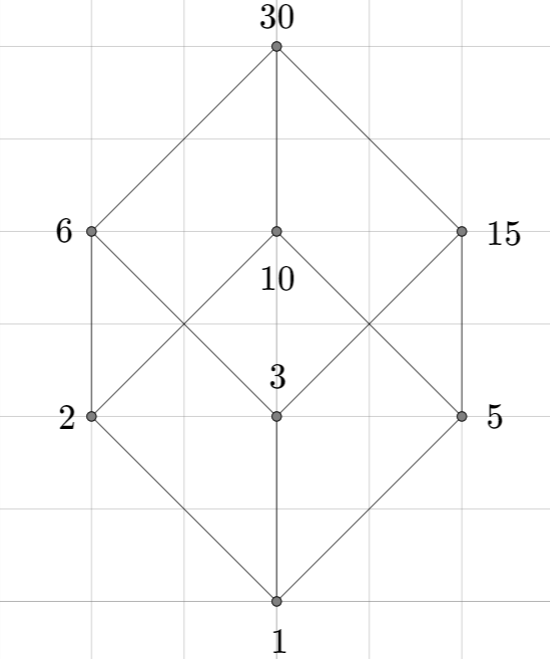
\includegraphics[width=0.4\textwidth]{images/hasse.png}
		\end{tabular}
		\begin{tabular}{c}
			%Your reference code for the next loading is:
%Note! There is a percentage sign at the beginning of the line!

%H8KLCAAvD8KRYQIDw6XCllFvwpwwDMOHwr8LfS3CkcKdw4ROw5zDj8KwSXsvfUDCg8KpaDfCqMOuwpDDmmrDosK7L8OkwrjDq3HCu8KtJ8KNwo4rBQnCgR3DssO3w492CMOJw63Djyxpwp8fw4oswrnDicKST8Kfw7PDtj5Lwq7Cs8Oka1PCt2XDnQZrw7Bvw5p1w7N9O8OiCsOiEcOHPAVLKsKKwrwjIMKDVhstaMKDw6M5OMKsU8KOw4LDvSpvw4vCp8O4KmZJw5ddw7/CoxxqwqvCjCfDklrCrBEPwqIHwr3DlBnCpcOHwoJ6EkFQwoHCjsOZChE7QMK/A0zChcKUwrEOwo0Xw41gwrUbacKbCcK0EVg5w5PCn8KAAmjDrAEqaS/DpBDCnGfDsCNlwpomw43CpDwzwockE3vCrcKjRsOUw4YgflRYwp5EwpEUe2RHFHgxSMK6wr3CosO1w4fClUV4w4vDtMKiw5PCilECf8K4OBbDocKxOE3DhMOrwq1BIMOnwoEFDcKYwp18wqjDrHHChsONCcOewqouw49WXMKFw4HCj1XDkcOHeAPDig7CliLDn8O0wobDm8K7w7BcVD/DinpTNcO1bsKefD1MOcKsAsOYZwfCoAvDt2VdwrzDuHdOw6h6V8K+XjfCjzHChjTCqsK3w5XDg2Y7w7bCvsOMwovDqBjDkHpnXsKtDk3DncKcwpwvHH8iwozDuEvChTzCqsOyw7vDhjzDrFl9wqJnw5PDhcOSw75twoXDhlQswqN/T3IeV33DgcKoIkrCiMKlw5/CpcO7fRPDvQF3w5jCvMKFPMOHPyTDsMO8w47Dk8OwcXrDuxXDkkU1w7crw5/Dp8K9w5MsZxnCm8KPw7PDhTLDv33CoX5pwqoew65Mw5Bvw5VqO8ObwpXCh8O+PMKTw75EZ8OOEsODw69dM3sYOF8YwpcUw4NsAVxGKS7Coy/DhzHDnCXCvwDDsMKRUkvDpxIAAA==

%Your TikZ code is as follows:
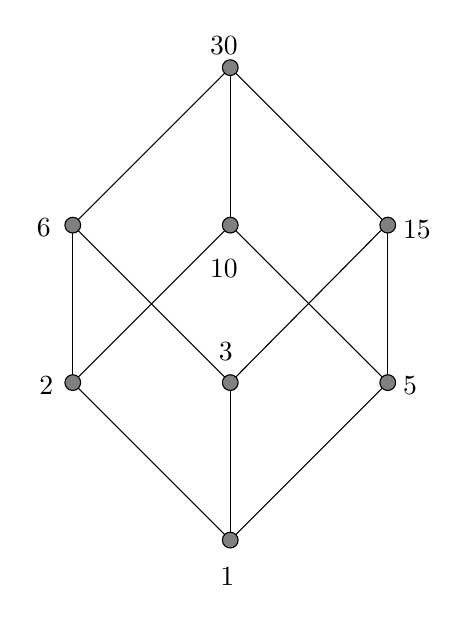
\begin{tikzpicture}
	\node[black, anchor=south west] at (-0.25,-0.70) {$1$};
	\node[black, anchor=south west] at (-2.55,1.72) {$2$};
	\node[black, anchor=south west] at (-0.27,2.16) {$3$};
	\node[black, anchor=south west] at (2.07,1.72) {$5$};
	\node[black, anchor=south west] at (-2.58,3.73) {$6$};
	\node[black, anchor=south west] at (-0.38,3.21) {$10$};
	\node[black, anchor=south west] at (2.07,3.70) {$15$};
	\node[black, anchor=south west] at (-0.38,6.04) {$30$};
	\draw[draw=black, thin, solid] (-2.00,2.00) -- (0.00,0.00);
	\draw[draw=black, thin, solid] (0.00,0.00) -- (0.00,2.00);
	\draw[draw=black, thin, solid] (0.00,0.00) -- (2.00,2.00);
	\draw[draw=black, thin, solid] (-2.00,4.00) -- (-2.00,2.00);
	\draw[draw=black, thin, solid] (-2.00,2.00) -- (0.00,4.00);
	\draw[draw=black, thin, solid] (0.00,2.00) -- (-2.00,4.00);
	\draw[draw=black, thin, solid] (0.00,2.00) -- (2.00,4.02);
	\draw[draw=black, thin, solid] (2.00,2.00) -- (0.00,4.00);
	\draw[draw=black, thin, solid] (2.00,2.00) -- (2.00,4.00);
	\draw[draw=black, thin, solid] (2.00,4.00) -- (0.00,6.00);
	\draw[draw=black, thin, solid] (0.00,6.00) -- (-2.00,4.00);
	\draw[draw=black, thin, solid] (0.00,6.00) -- (0.00,4.00);
	\draw[draw=black, fill=gray, thin, solid] (0.00,6.00) circle (0.1);
	\draw[draw=black, fill=gray, thin, solid] (-2.00,4.00) circle (0.1);
	\draw[draw=black, fill=gray, thin, solid] (-2.00,2.00) circle (0.1);
	\draw[draw=black, fill=gray, thin, solid] (0.00,2.00) circle (0.1);
	\draw[draw=black, fill=gray, thin, solid] (0.00,0.00) circle (0.1);
	\draw[draw=black, fill=gray, thin, solid] (2.00,2.00) circle (0.1);
	\draw[draw=black, fill=gray, thin, solid] (2.00,4.00) circle (0.1);
	\draw[draw=black, fill=gray, thin, solid] (0.00,4.00) circle (0.1);
\end{tikzpicture}

%File created at 2021. 11. 10. 0:19:07
		\end{tabular}
	\end{tabular}
	\caption{Egy Hasse-diagram az alkalmazásban és kimentve}
\end{figure*}

\Section{Általános gráf}

A gráf (vagy irányítatlan gráf) egy $G = (V, E)$ pár, ahol $V$ egy olyan halmaz, amelynek elemeit csúcsoknak, $E$ pedig a (rendezett) csúcspárok halmaza, amelynek elemeit éleknek nevezzük. Néha a gráfok tartalmazhatnak hurkokat, azaz olyan éleket, amelyek egy csúcsot önmagához kapcsolnak. Az ilyen általánosított gráfokat hurokkal rendelkező gráfoknak vagy egyszerűen gráfoknak nevezzük, ha a kontextusból egyértelmű, hogy a hurok megengedett.

\begin{figure}[!h]
	\label{fig:graph_editor}
	\centering
	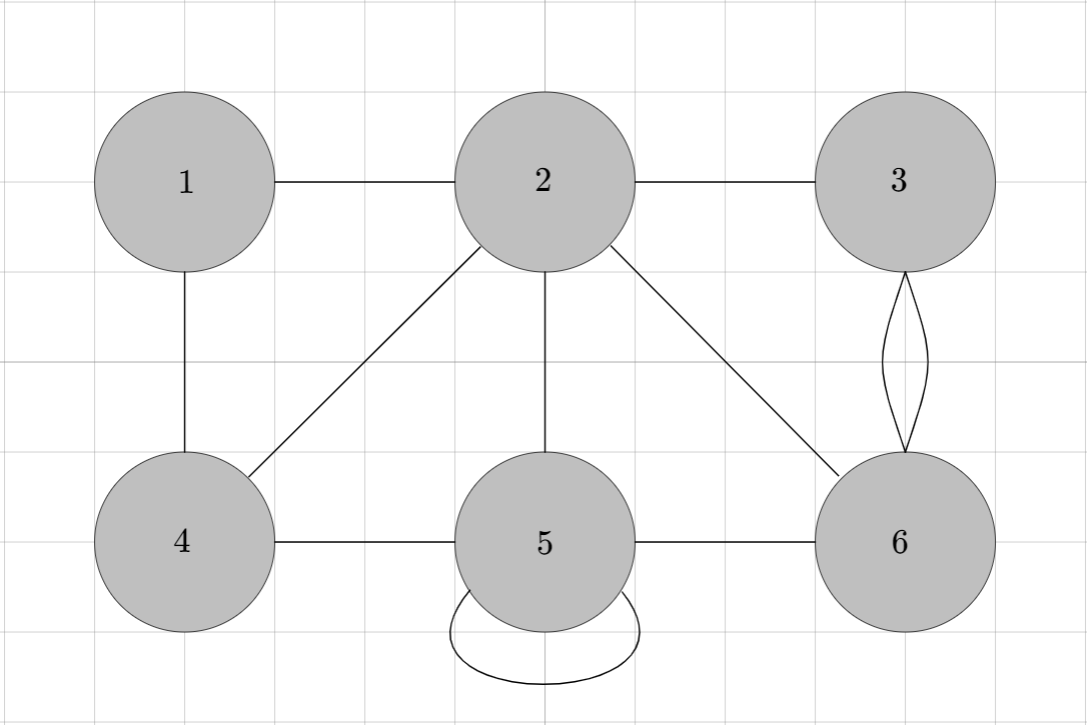
\includegraphics[width=0.75\textwidth]{images/graph.png}
	\caption{Egy gráf képe az alkalmazásban}
\end{figure}

\begin{figure}[!h]
	\label{fig:graph_tikz}
	\centering
	%Your reference code for the next loading is:
%Note! There is a percentage sign at the beginning of the line!

%H8KLCAAbEMKRYQIDw51Xw5vCjhpHEMO9F8O8w6oZdVV1XcOaworDssOgaMO9w6R8woHDlw8oTGQUAisWw4l2wqLDvcO3wpzDoTLCsMKwwowce0jClgUBQ8O3w5TCnDp1w6/DkcKHwr9vR8Krwq93w43DrcOow43DrcOoZjbCm8Oew53Do8O6w7XDrcOowrfDhXzDlcOMV1jDhx3Dt8Krw6XDosKPw409wq/DksO6wrXCvsOnw7fDqWzCtll8w7vCrn3Crxdnw5N5w7N5Oll9w4JOwqrDs3ZlMsK+bxc+fMOEw7/DicO0w49mfj9dw4x3Dx8vwrc4X8OwU2nDgj1fccKlw6kBV8ONfMKyw5/DrMO2CMKbeMK9fnbDqlPCn8O6fE3DulfDlMOLwqB6wq4Mwqp+BldAwoDDuxlUdFUcw7oZPMKVCMOvAcO1w43Dqj/DljTCvkPDk8OUwqfDqX53bWtcwo/Cl8OLw4XDp8K1Gj9Vaw1WMMO3RsOiUzPCnsKsd2bDo1XDs2XCsznCnsOODsKXw75fwq4Hdk9PwpB9wrTDu8KYa8O1w7PClXHDrXHDqnnCj14dw4vDg3LCncO6worDnQvDsGhvw6zDkkvCisOdwqrDn8KrFcK9KMK/VmTCuWZPXMK8ZGHDjcK6JWdSe8OOYcKUIsKIwrLCl1NLwojDlsOFw5lzwokkO8KTQCw4wqIwJ8OBwrfDpMKrT3LDo8K6JFHCiWwew6Faw7YGYsOhwpTCk8K6csOJfGogwrHDmgrCm1HCsHHDlsOiwp3CkXLCncKLwqrDonFJwrUkwr5Eb8O7dcOccsO+Rittw5otwqXCmlkECmnDshw5dgo7woLCoQ3CjC0WwoTCqUXDvHFAwq7CnXMqWsKCKXPDpF0ZYT0Gw4xDAALCjwwBa8OCWUjDjXLDhzAfA8OyIMKAw5QCwoJbEnLDtcKSwqJjaMOHwoA6ACDChcOWEsOBahnDoSUhw6fDucOJQHARIcOFLTHCkcKTHsOQw6PDh3h2woLDt8K2w7lrw5oswr9jVsK+KTfCv8OcwrwbwqbDvmXCqj3ChVBbwrDDsMOOBwQQwpMewplMwpMgw7NPw5I7wrfChUHCjcOQBRBTw67DksKJeh3DmTMrwpXDlMOWwowYwqIGbsKNwrRcw4zCtkJ3dFjDhVNCwqBFIMKXUG9QwpF5wqdMwrFaTcOFwpHDlWHDrGbDrcKTw654L1vCvGYTw4vCpkh9w6TChR5IJmVVFATCjcOkw6QnZ8KFw6fDoMOAw54TRMOfAWJ4L1BIwp0yTMKMwo4gaMKbwrJzAnzCo8KKw7TCgF/DhAl+KnrDrMKFfyXDu8K8w71Qw7U6w6I/w7ADExovw7puQcOnRQLCm8OtbFnDoTTCrQlDwonCiMKxwqJ5Cx3Du8KhwpUNw6cgw4HDuGLCocKue1kuw5o6wqAtBhDDjSQPD0N0CMK0wojCohnDgxfChgvDqMOUTQnCiAjCvkRLQsOCOxVMdlrDhMOdwrrCusKFwp7Di8KXw6jCucKtN8KKFRTCkWJaw7DDmRUYP8OGwqNhw7DDjhjClE4Bw7XCsj3CvsKcTDE+ACDDlwhfwoVFw4nDncOJEsOtw713woERJkotw6hxasOSHhLClMK6Lkd2wonDsETDkxETQh/CosKgUsKEw44Gw4sgw7PCi8KBXcK0w43DkVFgwqnDq33Cp8KpMERocgJaw4E0woHDo8KUMxheFMOtwpzDo8Kqw4hPDsOzH0fDvwDDrVVtwqbCkRgAAA==

%Your TikZ code is as follows:
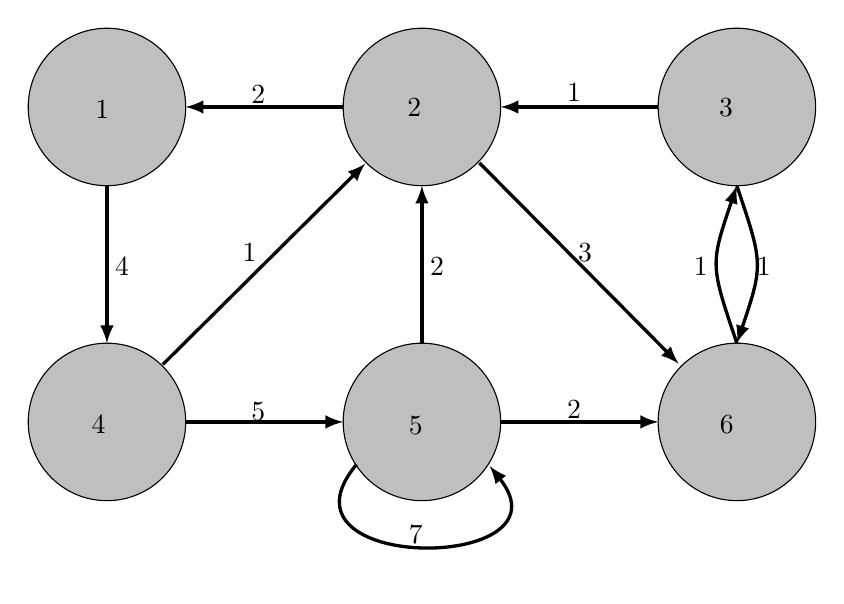
\begin{tikzpicture}
	\draw[draw=black, fill=lightgray, thin, solid] (0.00,-2.00) ellipse (1.00 and 1.00);
	\draw[draw=black, fill=lightgray, thin, solid] (4.00,-2.00) ellipse (1.00 and 1.00);
	\draw[draw=black, fill=lightgray, thin, solid] (4.00,2.00) ellipse (1.00 and 1.00);
	\draw[draw=black, fill=lightgray, thin, solid] (0.00,2.00) ellipse (1.00 and 1.00);
	\draw[draw=black, fill=lightgray, thin, solid] (-4.00,2.00) ellipse (1.00 and 1.00);
	\draw[draw=black, fill=lightgray, thin, solid] (-4.00,-2.00) ellipse (1.00 and 1.00);
	\draw[draw=black, latex-, very thick, solid] (-4.00,-1.00) -- (-4.00,1.00);
	\draw[draw=black, -latex, very thick, solid] (-3.00,-2.00) -- (-1.00,-2.00);
	\draw[draw=black, -latex, very thick, solid] (0.00,-1.00) -- (0.00,1.00);
	\draw[draw=black, -latex, very thick, solid] (3.00,2.00) -- (1.00,2.00);
	\draw[draw=black, -latex, very thick, solid] (1.00,-2.00) -- (3.00,-2.00);
	\draw[draw=black, -latex, very thick, solid] (-1.00,2.00) -- (-3.00,2.00);
	\draw[draw=black, -latex, very thick, solid] (-3.29,-1.27) -- (-0.72,1.28);
	\draw[draw=black, latex-, very thick, solid] (3.26,-1.26) -- (0.73,1.29);
	\node[black, anchor=south west] at (-4.27,1.73) {$1$};
	\node[black, anchor=south west] at (-4.32,-2.27) {$4$};
	\node[black, anchor=south west] at (-0.31,1.75) {$2$};
	\node[black, anchor=south west] at (-0.29,-2.29) {$5$};
	\node[black, anchor=south west] at (3.65,1.75) {$3$};
	\node[black, anchor=south west] at (3.66,-2.27) {$6$};
	\draw[draw=black, very thick, -latex, solid] (-0.83,-2.54) .. controls (-2.00, -3.93) and (1.95, -3.92) .. (0.86,-2.56);
	\draw[draw=black, very thick, -latex, solid] (4.00,-1.00) .. controls (3.66, -0.00) and (3.66, -0.00) .. (4.00,1.00);
	\draw[draw=black, very thick, -latex, solid] (4.00,1.00) .. controls (4.33, 0.01) and (4.34, 0.01) .. (4.00,-1.00);
	\node[black, anchor=south west] at (-2.29,1.92) {$2$};
	\node[black, anchor=south west] at (-4.02,-0.26) {$4$};
	\node[black, anchor=south west] at (-2.40,-0.09) {$1$};
	\node[black, anchor=south west] at (-2.29,-2.10) {$5$};
	\node[black, anchor=south west] at (-0.29,-3.67) {$7$};
	\node[black, anchor=south west] at (-0.02,-0.27) {$2$};
	\node[black, anchor=south west] at (1.72,-2.08) {$2$};
	\node[black, anchor=south west] at (1.86,-0.09) {$3$};
	\node[black, anchor=south west] at (3.33,-0.26) {$1$};
	\node[black, anchor=south west] at (4.13,-0.26) {$1$};
	\node[black, anchor=south west] at (1.72,1.95) {$1$};
\end{tikzpicture}

%File was created at 2021. 11. 10. 00:43:15
	\caption{Az alkalmazásból kimentett gráf képe}
\end{figure}

\Section{Folyamatábra}

A folyamatábra egy olyan diagramtípus, amely egy adott folyamatot vagy eljárást ábrázol. A folyamatábra definiálható úgy is, mint egy algoritmus, egy feladat megoldásának lépésről lépésre történő megközelítése.

Az folyamatábra a lépéseket különböző típusú dobozokként, a lépések sorrendjét pedig a dobozok nyilakkal való összekapcsolásával mutatja be. Ez a diagrammszerű ábrázolás egy adott probléma megoldási modelljét szemlélteti. A folyamatábrákat különböző területeken használják egy folyamat vagy program elemzése, tervezése, dokumentálása vagy kezelése során.

\begin{figure*}[!h]
	\label{fig:flowchart}
	\centering
	\begin{tabular}{c}
		\begin{tabular}{c}
			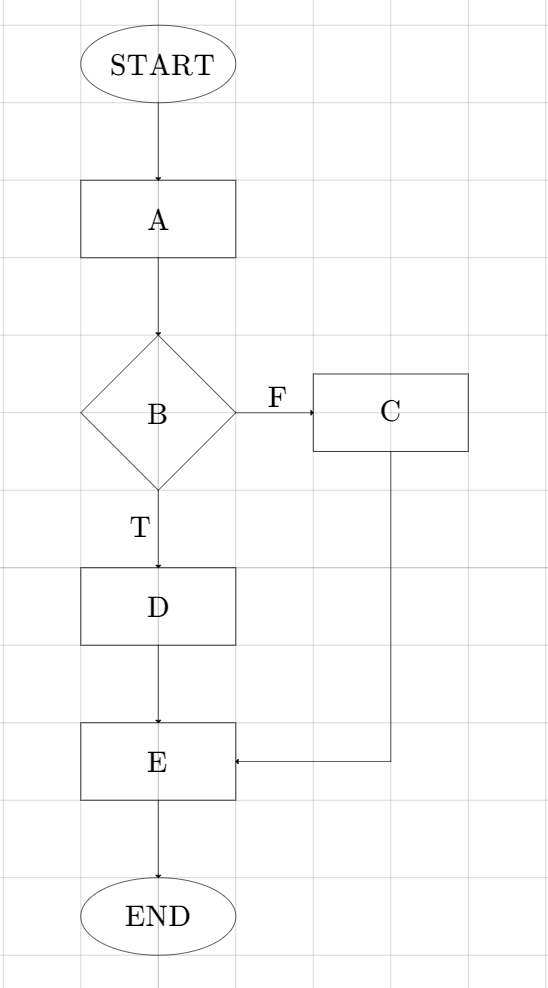
\includegraphics[width=0.45\textwidth]{images/flowchart.png}
		\end{tabular}
		\begin{tabular}{c}
				%Your reference code for the next loading is:
%Note! There is a percentage sign at the beginning of the line!

%H8KLCAAID8KRYQIDw6VXTW/DmzAMw70vw67CtREkShTCpWIYw5APw7c0w6zDkMOlVsO3YMOUw55qw5RzworDhEBbDMO5w69jwpwmwrFrw5dow5YEw4nDklzDosOwKXx6Ik1Sw4HDtcKfKCjCnx/Dkig4wonCgmHDulRGw4FxFMOcwo7CijItw7jDucKEw6FJOR7DncOPFxzDicOqU8KteWLDi0DCk0BAKR3CkHHCiEoxw7A8A8OAwpPCsMKKwqQjQMO0GjQyUlbDvsOZw4/Cj8Ohw6nDlTAKwqbDk8OjOsO9wrfCrEjDn03Cn8Ozw6LDhywpw68YwpHDgsK8WMKSeDIzXMOfw7DDryTDu8KdFsKTbFQsw7zDhMOjF8KXwrPCrcOLw4VOwrXClFN+TsKLwqQDZG3Dkxkawo/Dh8Kjw4dqD8KDwq8VfcKZPUzDpsOrw6/DkjjCqcKQPGZ9czDDjsOywrppw7pKaMKYw6fDvMO3w7drw73CmcOlc39HwqEPw4/Dg8OLwo0cw4AAV0fCgMOtI8OAw4YBwr1WcMKVw57ClnHDsSvDnx8Nw5DCqwE6NMOsJsOdwqAvw53DlFbDkm03QlVHQGrDsVLCsiXDtcKQwpQewpLDkMKmwpY3wpMXDybCoMKfJnPDscOtcG7CoxDDrUnDl8OgAC5jCcOYOgFYw4HChMK7w60aw7XCncOKw7XCisOMwpcNJMOlw7rDsyDDoCJ9w6rDo157w5Rbw5vCszVCS3JkwpXDsgbDjXLDjnRaWFJGWl7DjMOfworDqsK8wpcfw6cdKC3CkMKMwrbDhgPCkgPCtEtqw4Ujwq4Hw4dDLiFpC8Oew5XCuU9bw5x7NzPDtSQUw67DicK4w5RTwqA6w4rDsMOhwpTCqFXCkHrDn3vCtS9xUj3CgQLDuQnDrlDDkBcmw6gIw5M/w5RWEmTCuAZawq/CiMKAL8OcZsOpXgnDkMOOeMO0w5JrwqnCqVEEw4PDrxfCu8K9acKrVcK6dnTDmxVadcObw796wq7DqlfDmgA3w79CbMKywrURw7R0wrbCs8KPd1XCpcKtMMKgwqUxRkprw4DCuCXCsxHDqMKNw5PDhEYJwp4aw4zDp8Obw6zDpwjCgicIBx4MWE0Sw6rDjBfDm2RWwr3DlMOhwozDuibDuAvCicKVL8KSwqoTAAA=

%Your TikZ code is as follows:
\begin{tikzpicture}
	\node[black, anchor=south west] at (-0.81,6.20) {START};
	\draw[draw=black, -latex, thin, solid] (0.00,6.00) -- (0.00,5.00);
	\draw[draw=black, thin, solid] (0.00,6.50) ellipse (1.00 and 0.50);
	\draw[draw=black, thin, solid] (-1.00,5.00) rectangle (1.00,4.00);
	\draw[draw=black, -latex, thin, solid] (0.00,4.00) -- (0.00,3.00);
	\draw[draw=black, thin, solid] (0.00,3.00) -- (-1.00,2.00);
	\draw[draw=black, thin, solid] (0.00,3.00) -- (1.00,2.00);
	\draw[draw=black, thin, solid] (1.00,2.00) -- (0.00,1.00);
	\draw[draw=black, thin, solid] (0.00,1.00) -- (-1.00,2.00);
	\draw[draw=black, -latex, thin, solid] (0.00,1.00) -- (0.00,0.00);
	\draw[draw=black, thin, solid] (2.00,2.50) rectangle (4.00,1.50);
	\draw[draw=black, latex-, thin, solid] (2.00,2.00) -- (1.00,2.00);
	\node[black, anchor=south west] at (-0.56,0.25) {T};
	\node[black, anchor=south west] at (1.22,1.92) {F};
	\node[black, anchor=south west] at (-0.33,4.21) {A};
	\draw[draw=black, thin, solid] (-1.00,0.00) rectangle (1.00,-1.00);
	\draw[draw=black, -latex, thin, solid] (0.00,-1.00) -- (0.00,-2.00);
	\draw[draw=black, thin, solid] (-1.00,-2.00) rectangle (1.00,-3.00);
	\draw[draw=black, -latex, thin, solid] (0.00,-3.00) -- (0.00,-4.00);
	\draw[draw=black, thin, solid] (0.00,-4.50) ellipse (1.00 and 0.50);
	\node[black, anchor=south west] at (-0.62,-4.77) {END};
	\draw[draw=black, thin, solid] (3.00,-2.50) -- (3.00,1.50);
	\draw[draw=black, -latex, thin, solid] (3.00,-2.50) -- (1.00,-2.50);
	\node[black, anchor=south west] at (-0.33,1.71) {B};
	\node[black, anchor=south west] at (2.67,1.74) {C};
	\node[black, anchor=south west] at (-0.33,-0.79) {D};
	\node[black, anchor=south west] at (-0.33,-2.79) {E};
\end{tikzpicture}

%File was created at 2021. 11. 11. 14:28:40
		\end{tabular}
	\end{tabular}
	\caption{Egy folyamatábra képe az alkalmazásban és kimentve}
\end{figure*}

\Section{Nassi–Shneiderman-diagram}

A Nassi-Shneiderman-diagram a számítógépes programozásban a strukturált programozás grafikus ábrázolása. Isaak Nassi és Ben Shneidermann fejlesztette ki 1972-ben. Ezeket az ábrákat struktogramoknak is nevezik, mivel a program struktúráit mutatják.

A struktogramok a folyamatábra szabadosságát korlátozzák és csak struktúrált szimbólumokat tartalmaznak. Alapelem a téglalap, amit különböző módokon osztunk fel részekre. Maga a program egyetlen partícionált (felosztott) téglalap.

A Nassi-Shneiderman-diagramokat csak ritkán használják a formális programozásban. Absztrakciós szintjük közel áll a strukturált programkódhoz, és a módosítások miatt a teljes diagramot újra kell rajzolni. Az algoritmusokat és a magas szintű terveket egyértelművé teszik, ami az oktatásban is hasznossá teszi őket.

\begin{figure*}[!h]
	\label{fig:structogram}
	\centering
	\begin{tabular}{c}
		\begin{tabular}{c}
			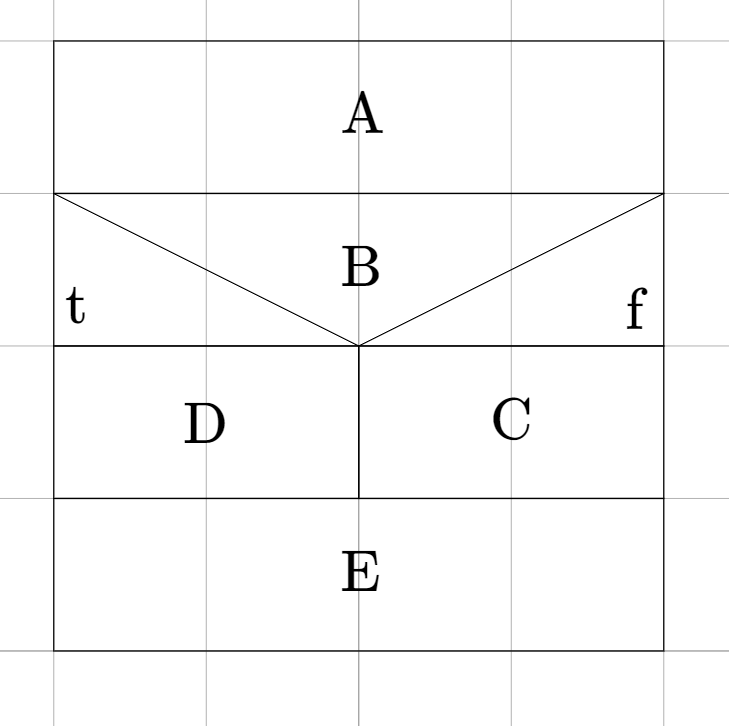
\includegraphics[width=0.3\textwidth]{images/structogram.png}
		\end{tabular}
		\begin{tabular}{c}
			%Your reference code for the next loading is:
%Note! There is a percentage sign at the beginning of the line!

%H8KLCAAaO8KRYQIDw5XCk1FPw5tADMKAw79LeMKlJ8Kfw493Z8OvbWPDnRNPaG/ClMKHwogcI1rClsKiw7YkwooQw799TkJLWsKxCsKJVsKDwrw0Z8K7w7nDvMOZSXHDuTgrw7LDg13CmhVfZsOFRcK6w45lw7vCq8ORw5PDqcKswrjCnsK3OcK1WTNawrPDjMKLw7nDr8Khw6oEw7rCq8KvwrnCqcKbZghOZXo2w73DkQfCm8K6TcO3dcKVbzUDwobCniNVwrnDrALCl1d6wq7Dqj/CqV3DlsOzdsO9w7Byw7HDjFnDqcKPBcOQwprCh8Ouw59PesKTw5rDqiU3eUlOPDzDqXXDusKhDcK6JncdNjktw7vCqAbDozl3bcO+w5PDgX8OwoVXw5bCsGPDuAksEMO2W8K8wrLCi3PChcK9WcOgw5gTw5/CnsK3HsOKw4VifsOfwrcxw6kbw4jDtcOdcijCv01lw5UnwpoywqfDlcKQLMOrZhzDusKvwqp7P8KOw53CnRzDmsO0Z1rDpTfCmw7Ci0HCgyFET8OgfcKEwohsNw3CkhhGJHZow4V5w7DDnSxyD8OQB33DrcOgR2PDiz7DtMK3Q8KgAU0Ua8KjOCdOW3BrNMKTw7ExBsKEAAzCrMO4MTrCvx/DjcOWIGHDgGDChcKJwqLDnTjCszcBWVxnwo3DnsOxFsO4w6YAw47DgRnDtmzCncKywonDhUtYwpPCiQ3CgsO4KMKiw4MmwrJbw5PDvsO+fsKyCybCkm5RwoAcwqDDpX7CnQNZDCkVw5BHwrLDqsKOY8Oyw5kxXzEwNkZvQ2QIJMOkPcOIwpg9w63DmFfDhV/CjkfCi2wGCQAA

%Your TikZ code is as follows:
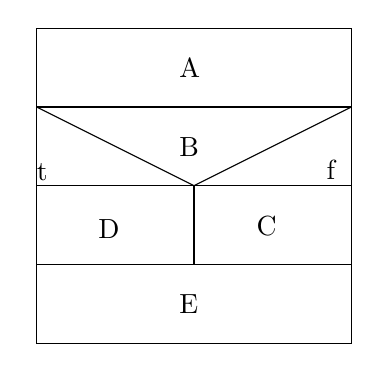
\begin{tikzpicture}
	\draw[draw=black, thin, solid] (2.00,0.00) rectangle (-2.00,1.00);
	\draw[draw=black, thin, solid] (2.00,1.00) rectangle (0.00,2.00);
	\draw[draw=black, thin, solid] (-2.00,2.00) rectangle (0.00,1.00);
	\draw[draw=black, thin, solid] (-2.00,3.00) rectangle (2.00,2.00);
	\draw[draw=black, thin, solid] (-2.00,4.00) rectangle (2.00,3.00);
	\draw[draw=black, thin, solid] (-2.00,3.00) -- (0.00,2.00);
	\draw[draw=black, thin, solid] (0.00,2.00) -- (2.00,3.00);
	\node[black, anchor=south west] at (-0.31,3.25) {A};
	\node[black, anchor=south west] at (-0.31,2.25) {B};
	\node[black, anchor=south west] at (-2.12,1.94) {t};
	\node[black, anchor=south west] at (1.56,1.96) {f};
	\node[black, anchor=south west] at (-1.34,1.21) {D};
	\node[black, anchor=south west] at (0.67,1.24) {C};
	\node[black, anchor=south west] at (-0.31,0.25) {E};
\end{tikzpicture}

%File was created at 2021. 11. 12. 17:34:49
		\end{tabular}
	\end{tabular}
	\caption{Egy struktogram képe az alkalmazásban és kimentve}
\end{figure*}